\documentclass{article}
\usepackage{graphicx}
\usepackage{tikz}
\usetikzlibrary{arrows,automata}


\begin{document}

\title{\huge{Boat Lift} \\ {\fontsize{13}{1} \selectfont Global requirements for the whole system} }
\author{Filippo Bernardi, Jasper Lustig, Jonas Wallmeier, Snorri Stefansson}

\maketitle

%\begin{abstract}

%\end{abstract}

\vspace{3cm}

\begin{figure}[!h]
\centering

	%\path[->, dashed]  (S)  edge              node {a} (l1);
	%\path[->, dotted]  (l1) edge [bend left]  node {a} (S);
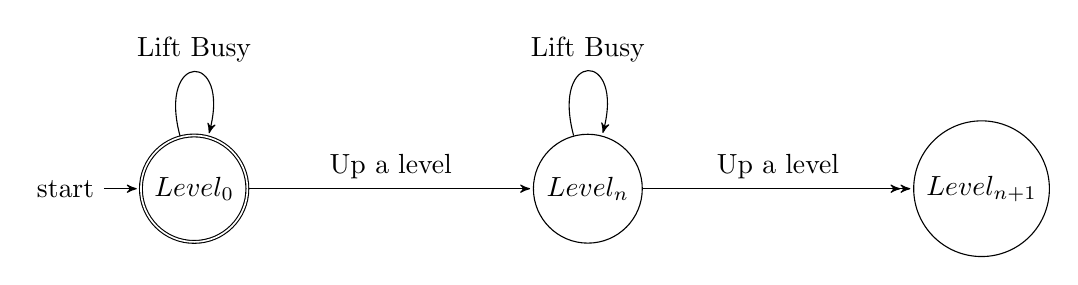
\begin{tikzpicture}[>=stealth',shorten >=1pt,auto,node distance=5cm]
	\node[initial,state,accepting] (S)      {$Level_0$};
	\node[state]         (l1) [right of=S]  {$Level_n$};
	\node[state]         (l2) [right of=l1] {$Level_{n+1}$};
		
	\path      (S)  edge [loop above] node {Lift Busy} (S);
	\path[->]  (S)	edge              node {Up a level} (l1);
	\path      (l1)	edge [loop above] node {Lift Busy} (l1);
	\path[->>] (l1) edge              node {Up a level} (l2);

	edge [bend left]  node {b} (l1);
\end{tikzpicture}
\caption{An extreme simple automata for the boat lift referenced in this document}
\end{figure}

\pagebreak

\section{}


If the assignment were about a bridge, typical requirements would be: ‘A bridge will never open when the barriers are not closed’; ‘If an operator instructs the bridge to open, the bridge will open unless the barriers are not closed’; and ‘A bridge will never open spontaneously’. These requirements are initially to be described in natural language. 

Definition:
Ship lift. General purpose ship lift for elevating ships to a geographically, vertical, higher location. 

Requirements for the whole system:
\begin{enumerate}
	\item Only one boat can be elevated at a time
	\item The lift has to be big enough for all boats going through.
	\item The water level in the lift can only change when both gates are closed securely.
	\item Gates should not close while a boat is going through them.
	\item The boats are signaled when to enter or leave the lift.
	\item Only one gate can be open at a time.
	\item Below every floor there has to be a valve.
	\item Every floor should be able to decrease its water level.
	\item The water flow can not distort the boats equilibrium.
	\item Sensing if the ship is completely inside the lift or not.
	
	
\end{enumerate}

A general requirement

\begin{enumerate}
	\item The gate should be open before the boats enters each floor
	\item After the boat is in the lift
\end{enumerate}

1–2. 	The boat enters the lock. 	
3. 		The lower gates are closed. 
4–5. 	The lock is filled with water from upstream. 	
6. 		The upper gates are opened. 	
7. 		The boat exits the lock. 	
8–9. 	The boat enters the lock.
10. 	The upper gates are closed.
11–12. 	The lock is emptied by draining its water downstream.
13. 	The lower gates are opened.
14. 	The boat exits the lock.
\pagebreak

Ask about:
Operator
Multiple floor.  More than one elevation 


\end{document}\grid
